% Vector reproduction of the diagram supplied by the team.
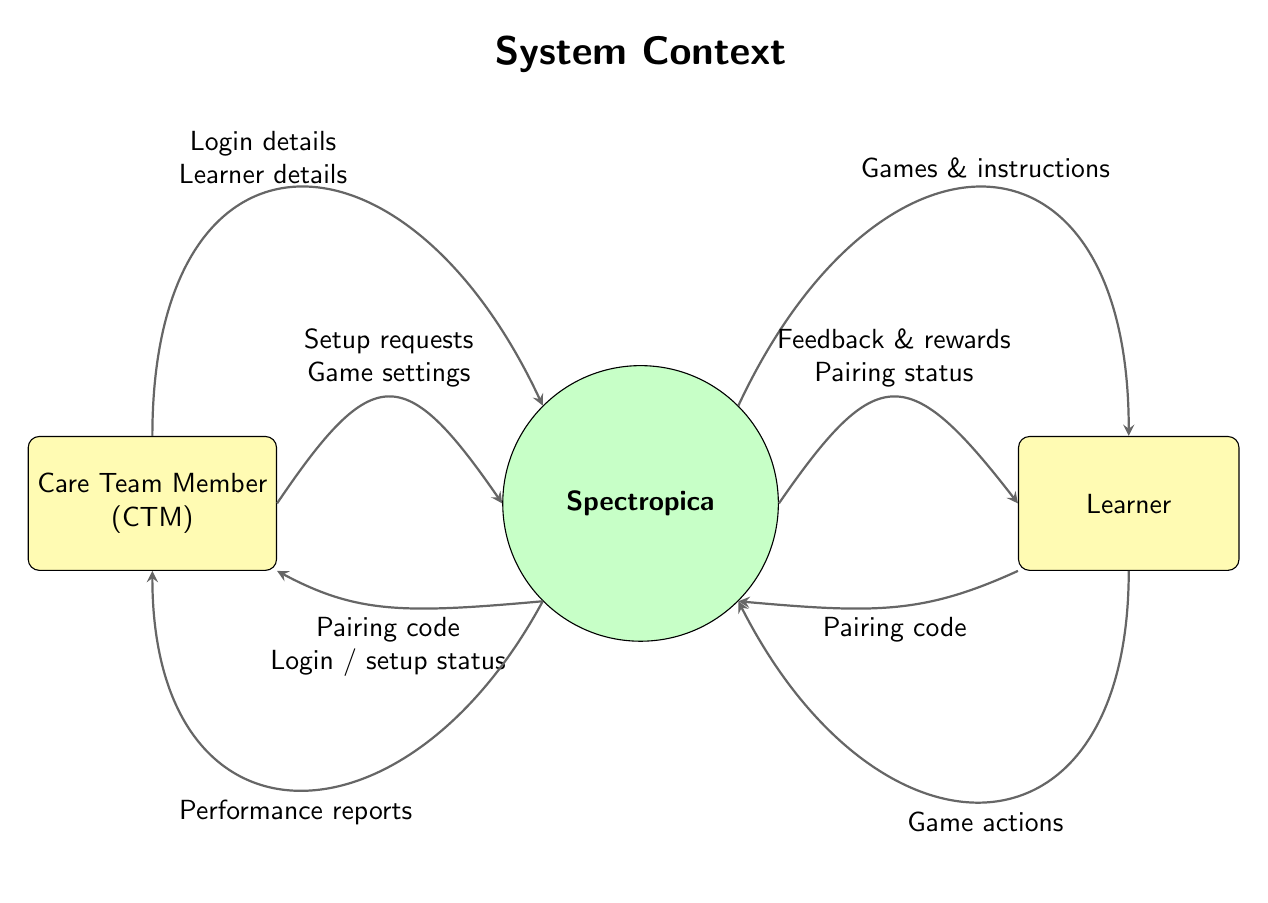
\begin{tikzpicture}[>=stealth,every node/.style={font=\sffamily,align=center},
flow/.style={->,draw=gray!80!black,thick}]
\node[font=\sffamily\bfseries\Large] at (0,5.7) {System Context};
\node[draw,fill=green!22,circle,minimum size=3.5cm,font=\sffamily\bfseries]
(s) at (0,0) {Spectropica};
\node[draw,rounded corners,fill=yellow!30,minimum width=2.8cm,
minimum height=1.7cm] (c) at (-6.2,0) {Care Team Member\\(CTM)};
\node[draw,rounded corners,fill=yellow!30,minimum width=2.8cm,
minimum height=1.7cm] (l) at (6.2,0) {Learner};
\draw[flow] (c.north) .. controls (-6.2,5) and (-3,5) .. (s.north west)
node[pos=.43,above] {Login details\\Learner details};
\draw[flow] (c.east) .. controls (-3.4,1.8) and (-3,1.8) .. (s.west)
node[pos=.5,above] {Setup requests\\Game settings};
\draw[flow] (s.south west) .. controls (-3,-1.4) and (-3.6,-1.4) ..
(c.south east) node[pos=.5,below] {Pairing code\\Login / setup status};
\draw[flow] (s.south west) .. controls (-3,-4.5) and (-6.2,-4.5) ..
(c.south) node[pos=.5,below] {Performance reports};
\draw[flow] (s.north east) .. controls (3,5) and (6.2,5) .. (l.north)
node[pos=.5,above] {Games \& instructions};
\draw[flow] (s.east) .. controls (3,1.8) and (3.4,1.8) .. (l.west)
node[pos=.5,above] {Feedback \& rewards\\Pairing status};
\draw[flow] (l.south west) .. controls (3.6,-1.4) and (3,-1.4) ..
(s.south east) node[pos=.5,below] {Pairing code};
\draw[flow] (l.south) .. controls (6.2,-4.7) and (3,-4.7) ..
(s.south east) node[pos=.5,below] {Game actions};
\end{tikzpicture}
